\documentclass[notes=hide,hyperref={dvipdfmx,pdfpagelabels=false}]{beamer}
\title{Einführung in Matlab - Einheit 3}
\subtitle{Rekursionen, Grafik}
\mode<article>
{
  \usepackage{fullpage}
  \usepackage{pgf}
  \usepackage{hyperref}
  \setjobnamebeamerversion{beamer}
}

\mode<presentation>
{
  %\usetheme{Frankfurt}
 %\usetheme{My}
  \usetheme{Madrid}
  % or ...
%\usecolortheme{seagull}
  %\setbeamercovered{transparent}
  %\setbeamercovered{dynamic}
  % or whatever (possibly just delete it)
}
\usenavigationsymbolstemplate{}
\usefonttheme{structurebold}
\usepackage{multimedia}
\usepackage{tikz}
\usepackage{fontspec,xunicode,xltxtra}
%\usepackage[scaled=.90]{helvet}
% Or whatever. Note that the encoding and the font should match. If T1
% does not look nice, try deleting the line with the fontenc.

\setbeamertemplate{footline}
{
\leavevmode
%\hbox{\begin{beamercolorbox}[wd=.5\paperwidth,ht=2.5ex,dp=1.125ex,
%leftskip=.3cm plus1fill,rightskip=.3cm]{author in head/foot}%
%    \usebeamerfont{author in head/foot}\insertshortauthor
%  \end{beamercolorbox}%
%  \begin{beamercolorbox}[wd=.5\paperwidth,ht=2.5ex,dp=1.125ex,leftskip=.3cm,
%rightskip=.3cm plus1fil]{title in head/foot}%
%    \usebeamerfont{title in head/foot}\insertshorttitle\hfill

\hfill\insertframenumber  \hspace{3pt}

%\inserttotalframenumber
%\hspace*{2ex}
%  \end{beamercolorbox}}%
  \vskip3pt%
}

%\usepackage[english]{babel}
\usepackage[ngerman]{babel}
\selectlanguage{ngerman}

%
% math/symbols
%
\usepackage{amssymb}
\usepackage{amsthm}
% \usepackage{latexsym}
\usepackage{amsmath}
%\usepackage{listings}
\usepackage[framed]{mcode}
%\usepackage{mcode}

\usepackage{mydef}
\usepackage{cmap} % you can search in the pdf for umlauts and ligatures
%\usepackage{colonequals} %corrects the definition-symbols \colonequals (besides others)
\title{Einführung in Matlab}
%
%\subtitle{Disputation} % (optional)

\author{Jochen Schulz}
% - Use the \inst{?} command only if the authors have different
%   affiliation.

\institute{Georg-August Universit\"at G\"ottingen \pgfimage[height=0.5cm]{../figures/unilogo3}}
% - Use the \inst command only if there are several affiliations.
% - Keep it simple, no one is interested in your street address.

\date{\today}

\subject{Einführung in Matlab}
% This is only inserted into the PDF information catalog. Can be left
% out. 



% If you have a file called "university-logo-filename.xxx", where xxx
% is a graphic format that can be processed by latex or pdflatex,
% resp., then you can add a logo as follows:

%\logo{\pgfimage[height=0.5cm]{figures/unilogo3}}


% Delete this, if you do not want the table of contents to pop up at
% the beginning of each subsection:
% \AtBeginSubsection[]
% {
%   \begin{frame}<beamer>
%     \frametitle{Aufbau}
%     \tableofcontents[currentsection,currentsubsection]
%   \end{frame}
% }

\AtBeginSection[]
{
  \begin{frame}<beamer>
    \frametitle{Aufbau}
    \tableofcontents[currentsection,currentsubsection]
  \end{frame}
}


\begin{document}



\maketitle


\section{Rekursionen}
%
% Slide
% 
\begin{frame}[fragile]\frametitle{Rekursive Funktionen}
Rekursive Funktionen sind Funktionen, die sich selbst aufrufen.\\
Bei jedem Aufruf wird ein neuer lokaler Workspace erzeugt.\\[1cm]

\textbf{Beispiel:} Fakult"at: $n!=\fak(n)$\\
\begin{eqnarray*}
 n!& = & n(n-1)!=n \fak(n-1)\\
& = & n(n-1)\fak(n-2)\\
& = & \cdots= n(n-1)\cdots 1 
\end{eqnarray*}
\end{frame}
%
% Slide
%
\begin{frame}[fragile]\frametitle{Fakult"at - rekursiv}
\lstinputlisting{fak.m}
\end{frame}
%
% Slide
%
\begin{frame}[fragile]\frametitle{Fakult"at - direkt}
\lstinputlisting{fak_it.m}
\end{frame}
%
% Slide
%
\begin{frame}[fragile]\frametitle{Fakult"at - Zeitvergleich}
\lstinputlisting{fak_vergleich.m}
\end{frame}
%
% Slide
%
\begin{frame}[fragile]\frametitle{rekursive Implementierung GGT}
\lstinputlisting{ggt_rekursiv.m}
\end{frame}
%
% Slide
% 
\begin{frame}[fragile]\frametitle{Sierpinski Dreieck}
\begin{itemize}
\item Wir beginnen mit einem Dreieck mit Eckpunkten $P_a$, $P_b$ und $P_c$. 
\item Wir entfernen daraus das Dreieck, das durch die Mittelpunkte der
  Kanten entsteht.
\item Die verbliebenden drei Dreiecke werden der gleichen Prozedur
  unterzogen.
\item Diesen Prozess können wir rekursiv wiederholen.
\item Das Ergebnis ist das Sierpinski Dreieck.
\end{itemize}
\end{frame}
%
% Slide
% 
\begin{frame}[fragile]\frametitle{Sierpinski Dreieck}
\begin{minipage}{5cm}
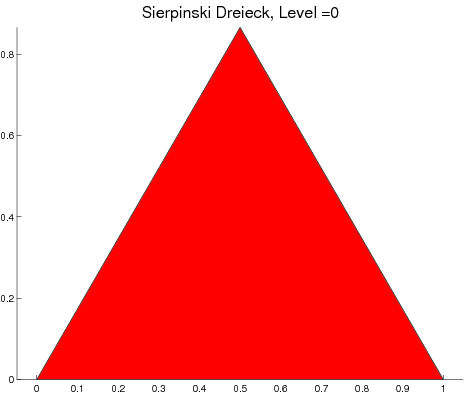
\includegraphics[height=4cm]{figures/sierpinski_0}
\end{minipage} \hfill
\begin{minipage}{5cm}
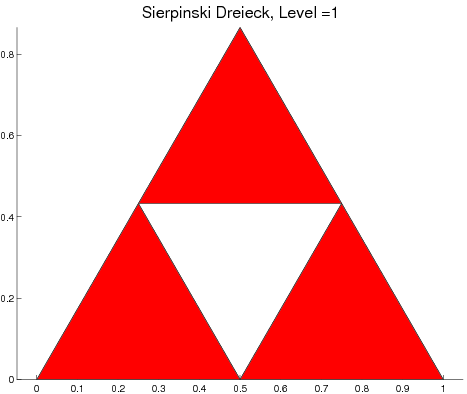
\includegraphics[height=4cm]{figures/sierpinski_1}
\end{minipage}\\ 
\begin{minipage}{5cm}
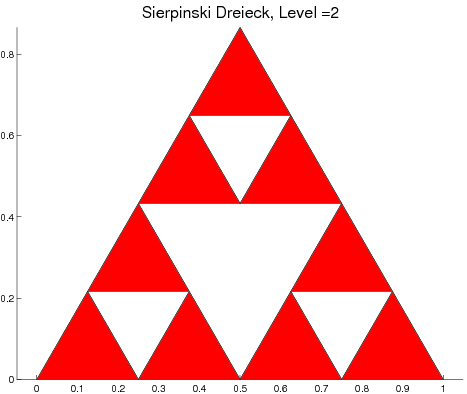
\includegraphics[height=4cm]{figures/sierpinski_2}
\end{minipage} \hfill
\begin{minipage}{5cm}
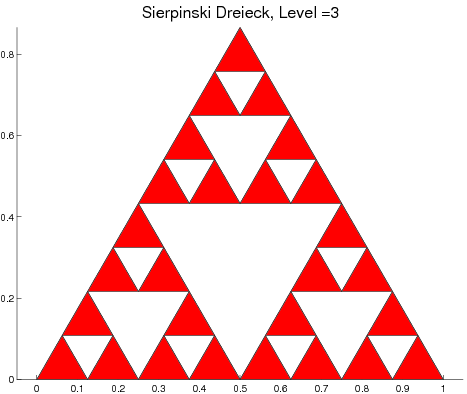
\includegraphics[height=4cm]{figures/sierpinski_3}
\end{minipage} \\
\end{frame}
%
% Slide
%
\begin{frame}[fragile]\frametitle{Implementierung}
\lstinputlisting{sierpinski_plot.m}
\end{frame}
%
% Slide
%
\begin{frame}[fragile]\frametitle{Implementierung}
\lstinputlisting{sierpinski.m}
\end{frame}
% 
% Slide
% 
\begin{frame}[fragile]\frametitle{Zeichnen von Polygonen}

Ein Polygon sei durch die Eckpunkte $(x_i,y_i)_{i=1}^n$ gegeben. Dann
kann er in MATLAB durch den Befehl
\begin{lstlisting}
fill(x,y,char)
\end{lstlisting}
dargestellt werden. \mcode{char} gibt die Farbe des Polygons an, z.B. rot
wäre 'r'.
\end{frame}


\section{Einf\"uhrung Grafik}
\subsection{einfache zweidimensionale Grafiken}
% 
% Slide
% 
\begin{frame}[fragile]\frametitle{Standard-Plot}
\begin{lstlisting}
plot(<x>,<y>)
\end{lstlisting}
zeichnet für Vektoren $x=(x_1, \ \dots \ ,x_N)$ und  $y=(y_1, \dots \ ,y_N)$
eine Grafik, die die Punkte $(x_i,y_i)$ und $(x_{i+1},y_{i+1})$ miteinander
verbindet.

\begin{columns}[c]
 \column{0.45\textwidth}
\textit{Beispiel:}
\begin{lstlisting}
x = linspace(0,2*pi,100);
y1 = sin(3*x);
plot(x,y1)
\end{lstlisting}
 \column{0.5\textwidth}
\pgfimage[width=\textwidth]{figures/grafik_1}
\end{columns}
\end{frame}
% 
% Slide
% 
\begin{frame}[fragile]\frametitle{Erweiterungen}
\begin{lstlisting}
plot(<x>,<y>,<string>)
\end{lstlisting}
\alert{String} besteht aus drei Elementen, die die Farbe, Linienstil
und die Markierung der Punkte kontrollieren. Die Reihenfolge der drei
Elemente ist beliebig.
\begin{columns}[c]
 \column{0.4\textwidth}
\textit{Beispiel:} Durch \\
\begin{lstlisting}
plot(x,y,'r*--') 
\end{lstlisting}
wird die Linie
gestrichelt (- -) in rot (r) gezeichnet und die Punkte durch *
markiert.
\column{0.55\textwidth}
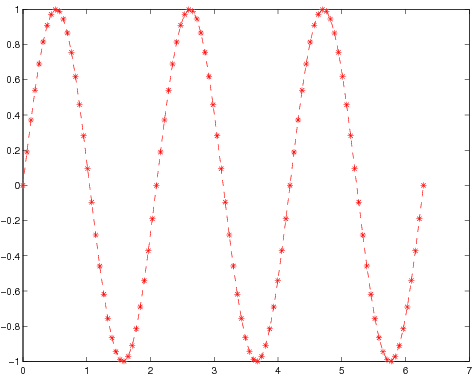
\includegraphics[width=\textwidth]{figures/grafik_2}
\end{columns}
\end{frame}
% 
% Slide
% 
\begin{frame}[fragile]\frametitle{Optionen}
\begin{tabular}{cp{8.5cm}}
\alert{ Farben} & r (rot), g (grün), b (blau), c (hellblau), m (magenta),
  y (gelb), k (schwarz), w (weiß)\\
\alert{ Marker} & o (Kreis), * (Stern), . (Punkt), + (Plus), x (Kreuz), s
  (Quadrat), d (Raute),... \\
\alert{ Linien-Stil} &  - (durchgezogene Linie), \mcode{--} (gestrichelte
  Linie), \mcode{:} (gepunktete Linie), \mcode{-.} (Strich-Punkt Linie)\\
\end{tabular}

Läßt man den Linien-Stil weg, so werden die Punkte nicht verbunden.
\end{frame}

% 
% Slide
% 
\begin{frame}[fragile]\frametitle{Optionen II}
\begin{lstlisting}
plot(<x>,<y>,<string>,<Eigenschaft>, <Spez.>) 
\end{lstlisting}
\alert{ Eigenschaften:}\\
\mcode{'MarkerSize'} (Default 6), \mcode{'LineWidth'} (Default 0.5),
\mcode{'MarkerEdgeColor'}, \mcode{'MarkerFaceColor'}\\

\begin{columns}[c]
 \column{0.6\textwidth}
\textit{Beispiel:} \\
\begin{lstlisting}
plot(x,y1,'b-.d','LineWidth',...
3,'MarkerEdgeColor','g')
\end{lstlisting}
\column{0.4\textwidth}
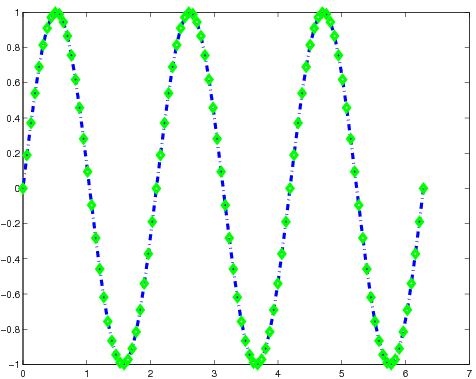
\includegraphics[width=\textwidth]{figures/grafik_3}
\end{columns}
\end{frame}
% 
% Slide
% 
\begin{frame}[fragile]\frametitle{Alternativen}
\begin{itemize}
\item Mehrere Plots in eine Grafik:
\begin{lstlisting}
plot(x1,y1,string1,x2,y2,string2,...) 
\end{lstlisting}
\item Logaritmische Skalierung in $x$- bzw in $y$-Richtung:
\begin{lstlisting}
semilogx(x1,y1) 
\end{lstlisting}
  bzw. 
\begin{lstlisting}
semilogy(x1,y1) 
\end{lstlisting}
\item Logarithmische Skalierung beider Achsen: 
\begin{lstlisting}
loglog(x1,y1)
\end{lstlisting}
\item Ist $X$ ein Vektor mit komplexen Einträgen, so ergibt \alert{
  \mcode{plot(X)}} 
\begin{lstlisting}
plot(real(X),imag(X))
\end{lstlisting}
\end{itemize}
\end{frame}
% 
% Slide
% 
\begin{frame}[fragile]\frametitle{Beispiel - Legendre Polynome}
%\begin{columns}[c]
% \column{0.52\textwidth}
\begin{lstlisting}[basicstyle=\scriptsize]
x = linspace(-1,1,100);
p1 = x;
p2 = (3/2)*x.^2-1/2;
p3 = (5/2)*x.^3-(3/2)*x;
p4 = (35/8)*x.^4 - (15/4)*x.^2+3/8;
plot(x,p1,'r:',x,p2,'g--',x,p3,'b-.',x,p4,'m-','LineWidth',2)
\end{lstlisting}
%\column{0.48\textwidth}
\hfil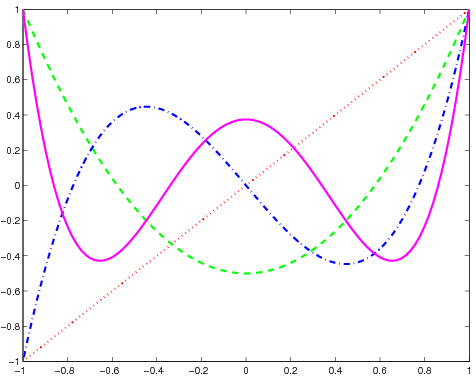
\includegraphics[width=0.55\textwidth]{figures/grafik_4}\hfil
%\end{columns}
\end{frame}
% 
% Slide
% 
\begin{frame}[fragile]\frametitle{Achseneinstellungen}
\begin{tabular}{p{4cm}p{7cm}}
\mcode{axis([x1 x2 y1 y2])} & Setzen der $x$- und $y$-Achsen
Grenzen\\
\mcode{axis auto} & Rückkehr zu Default Achsen Grenzen\\
\mcode{axis equal} & Gleiche Dateneinheiten auf allen Achsen\\
\mcode{axis off} & Enfernen der Achsen\\
\mcode{axis square} & quadratische Achsen-Box\\
\mcode{axis tight} & Achsen Grenzen werden passend zu den Daten
gewählt. \\
\mcode{xlim([x1 x2])} & Setzen der $x$-Achse\\
\mcode{ylim([y1 y2])} & Setzen der $y$-Achse\\
\mcode{grid on} & Gitter aktivieren\\
\mcode{box on}, \mcode{box off}  & Box um die Grafik
legen, Box entfernen
\end{tabular}
\end{frame}


\subsection{Beschriftungen}
% 
% Slide
% 
\begin{frame}[fragile]\frametitle{Beschriften der Grafik}
\begin{itemize}
\item Titel:  \alert{ \mcode{title('Titel')}}
\item Achsenbeschriftung:  \alert{ \mcode{xlabel('Text')}},
  \alert{ \mcode{ylabel('Text')}} 
\item Legende: \alert{ \mcode{legend('Text1','Text2',...,nr)}} \\
{\scriptsize \alert{ nr} gibt die Position der Legendenbox in der Grafik an:
  -1 (rechts vom Plot), 0 'bester' Ort, 1 oben rechts (default), 2
  oben links, 3 unten links, 4 unten rechts. }
\item zusätzlicher Text: \alert{ \mcode{text(x,y,'Text')}} Plaziert
  'Text' an die Position $(x,y)$ bzgl. der Werte auf der $x$-
  bzw. $y$-Achse. 
\end{itemize}
\end{frame}
% 
% Slide
% 
\begin{frame}[fragile]\frametitle{Bemerkungen zur Beschriftung}
\begin{itemize}
\item  In den strings kann direkt eine abgespeckte \LaTeX-Notation verwendet werden. (nahezu vollständige 
\LaTeX-Unterstützung: latex-interpreter).
Beispiele: 
\begin{itemize} \item \mcode{\\alpha} $\Rightarrow$ $\alpha$
\item \mcode{sin^\{3/2\}(x)} $\Rightarrow$ $\sin^{3/2}(x)$ .
\item \mcode{title('f(x) = \\frac\{1\}\{x^2+a\}','interpreter','latex')}
$\Rightarrow$ $f(x) = \frac{1}{x^2+a}$
\end{itemize}
\item Ändern der Schriftgröße, z.B. \mcode{title('Titel','FontSize', 20)}.
\item Auflistung aller modifizierbaren Texteigenschaften: \mcode{doc text_props}
\end{itemize}
\end{frame}
% 
% Slide
% 
\begin{frame}[fragile]\frametitle{Beispiel - Legendre Polynome II}
\begin{lstlisting}[basicstyle=\scriptsize]
title('Legendre Polynome','FontSize', 20)
xlabel('x','FontSize', 20)
text(0,0.45,'Maximum')
legend('n=1','n=2','n=3','n=4',4)
grid on, box on;
xlim([-1.1,1.1])
\end{lstlisting}
\hfil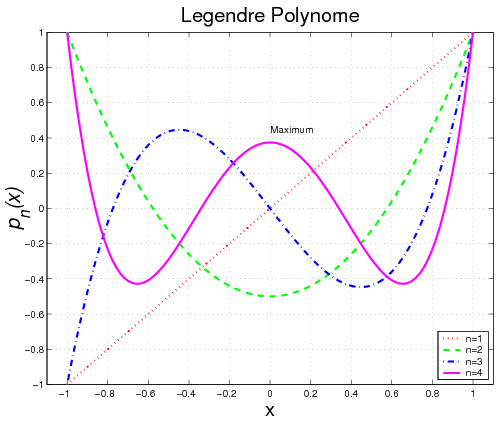
\includegraphics[width=0.5\textwidth]{figures/grafik_5}\hfil
%\end{columns}
\end{frame}
% 
% Slide
% 
\begin{frame}[fragile]\frametitle{Umgang mit Grafikfenster}
\begin{itemize}
\item Öffnen eines (weiteren) Grafikfensters: \alert{\mcode{figure}}.  Eine
  Grafik wird immer im aktuellen Fenster erzeugt. Ist noch kein
  Fenster geöffnet, so wird ein Fenster erzeugt.
\item Durch den Befehl \alert{\mcode{hold on}} werden bestehende Grafiken im
  aktuellen Fenster erhalten. Neue Grafiken werden den bestehenden
  hinzugefügt. 
\item \alert{\mcode{hold off}} (default) überschreibt Grafiken im
  aktuellen Fenster
\item Schliessen: \alert{\mcode{close}}, \alert{\mcode{close all}}
\end{itemize}
\end{frame}


\subsection{Weitere zweidimensionale Darstellungsmöglichkeiten}

% 
% Slide
% 
\begin{frame}[fragile]\frametitle{Darstellung von Daten}
\begin{itemize}
\item Balkendiagramm:
\begin{lstlisting}
bar(<Daten>) 
\end{lstlisting}
\item Histogramm: 
\begin{lstlisting}
hist(<Daten>,<Anzahl Bars>)
\end{lstlisting}
\item einfacher ausgefüllter Plot: 
\begin{lstlisting}
area(<x>,[<y1>,<y2>])
\end{lstlisting}
(y1 und y2 werden addiert)
\item Tortengrafik: 
\begin{lstlisting}
pie3([<anteil1> <anteil2> .. <anteilx>])
\end{lstlisting}
\end{itemize}
\end{frame}
% 
% Slide
% 
\begin{frame}[fragile]\frametitle{Darstellung von Daten}
\begin{center}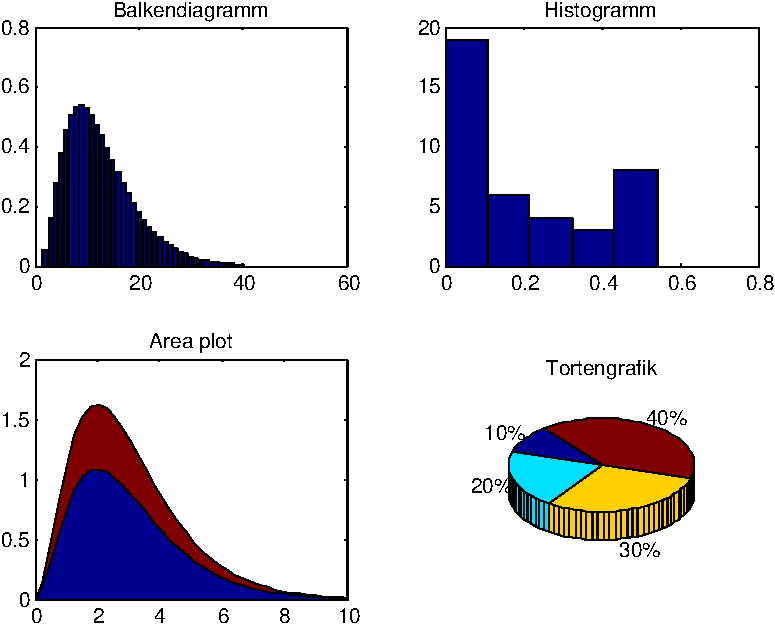
\includegraphics[height=0.8\textheight]{figures/darstellung_daten_2d}\end{center}
\end{frame}
% 
% Slide
% 
\begin{frame}[fragile]\frametitle{Darstellung von Daten}
\begin{lstlisting}
n = linspace(0,10,40);
y = n.^2.*exp(-n);

% Balkendiagramm
subplot(2,2,1),
bar(y); title('Balkendiagramm');

% Histogramm
subplot(2,2,2),
hist(y,5); title('Histogramm');

% Area plot
subplot(2,2,3),
area(n,[y',2*y']); title('Area plot');

% Tortengrafik
subplot(2,2,4),
pie3([ 1 2 3 4]); title('Tortengrafik');
\end{lstlisting}
\end{frame}
% 
% Slide
% 
\begin{frame}[fragile]\frametitle{Approximation von Integralen}
Approximiere $\int_0^1 f(x) dx$ durch
{\scriptsize \[ \int_0^1 f(x) dx \approx  \sum_{i=1}^{N} \frac{1}{N} f \left(
\frac{i-\frac{1}{2}}{N} \right ) \]}
für gegebenes $N \in \mathbb{N}$. \textbf{Beispiel}: $f(x)=x^3$
\begin{columns}[t]
\column{0.5\textwidth}
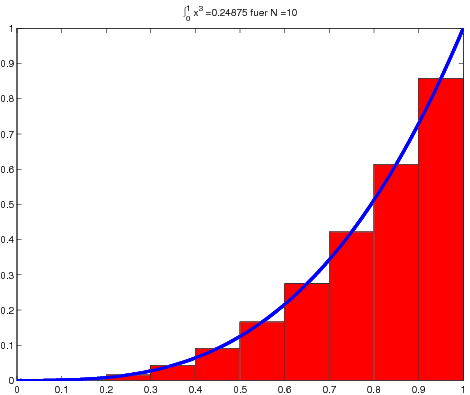
\includegraphics[width=\textwidth]{figures/integral_N=10} 
\column{0.5\textwidth}
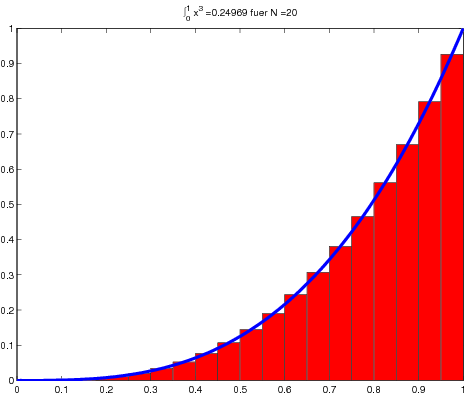
\includegraphics[width=\textwidth]{figures/integral_N=20}
\end{columns}
\end{frame}
% 
% Slide
% 
\begin{frame}[fragile]\frametitle{Integral - Implementation}
\lstinputlisting{integral.m}
\end{frame}

\subsection{Dreidimensionale Grafiken}

% 
% Slide
% 
% 
\begin{frame}[fragile]\frametitle{Dreidimensionale Grafiken}
\begin{itemize}
\item Dreidimensionale Version von \mcode{plot}: \alert{ \mcode{plot3}}
\item Darstellung von Funktionen $f:\mathbb{R}^2 \ \rightarrow \
  \mathbb{R}$:
\begin{itemize}
\item Contourplot (zeichnet die Niveaulinien): \alert{ \mcode{contour}}, \alert{
    \mcode{contourf}}, \alert{ \mcode{contour3}}
\item Darstellung des Graphen mit Gitterlinien: \alert{ \mcode{mesh} ,
  \mcode{meshc}} 
\item Flächige Darstellung des Graphen: \alert{ \mcode{surf}, \mcode{surfc}}
\end{itemize} 
\item Darstellung von Funktionen $f:\mathbb{R}^3 \ \rightarrow \
  \mathbb{R}$:
\begin{itemize}
\item Streifenansichten \alert{ \mcode{slice}}
\end{itemize}
\end{itemize}
\end{frame}

% 
% Slide
% 
\begin{frame}[fragile]\frametitle{plot3}
Bei gegebenen Vektoren $x=(x_i)_{i=1}^n$, $y=(y_i)_{i=1}^n$,
$z=(z_i)_{i=1}^n$ erzeugt \alert{ \mcode{plot3(x,y,z)}} einen Plot der die Punkte
$(x_i,y_i,z_i)$ und $(x_{i+1},y_{i+1},z_{i+1})$ miteinander
verbindet. \\
\begin{center}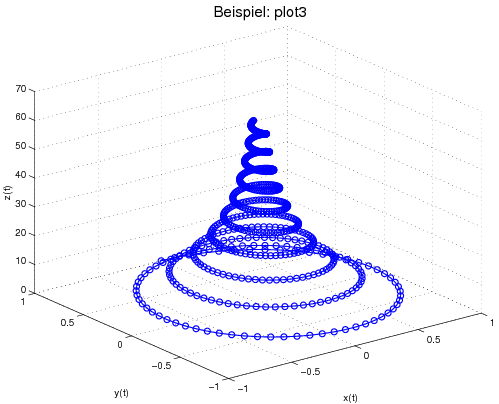
\includegraphics[width=0.6\textwidth]{figures/beispiel_plot3}\end{center}
\end{frame}
% 
% Slide
% 
\begin{frame}[fragile]\frametitle{Beispiel plot3}
\begin{lstlisting}
t = 0:0.1:20*pi;
x = exp(-t/20).*sin(t);
y = exp(-t/20).*cos(t);
z = t;

plot3(x,y,z,'b-o','LineWidth',1);
grid on
xlabel('x(t)'), ylabel('y(t)');
 zlabel('z(t)');
title('Beispiel: plot3','FontSize',15);
\end{lstlisting}
\end{frame}
% 
% Slide
% 
\begin{frame}[fragile]\frametitle{Blickwinkel}
\centering\alert{ \mcode{view(az,el)}}
\begin{itemize}
\item \alert{ \mcode{az}} ist die horiz. Rotation in Grad (Def. \alert{
  $-37.5$}) 
\item \alert{ \mcode{el}} ist die vertikale Rotation in Grad (Def. \alert{
  $30$})
\end{itemize}
\begin{center}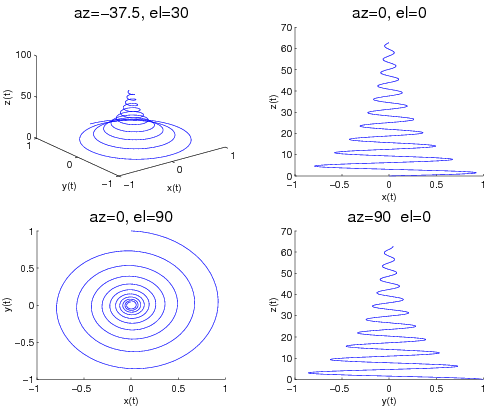
\includegraphics[width=0.6\textwidth]{figures/beispiel_plot3_2}\end{center}
\end{frame}
% 
% Slide
% 
\begin{frame}[fragile]\frametitle{3D-Funktionenplots}

Darstellung von Funktionen
\[ f: \mathbb{R}^2 \quad  \rightarrow \quad \mathbb{R} \]
\hspace*{1cm}\\

\textbf{Beispiel:}\\
\alert{ \[ f(x,y):=\exp(-x^2-y^2)\sin(\pi x y) \]}
\end{frame}
% 
% Slide
% 
\begin{frame}[fragile]\frametitle{Beispiel: Funktionenplot}
\hfil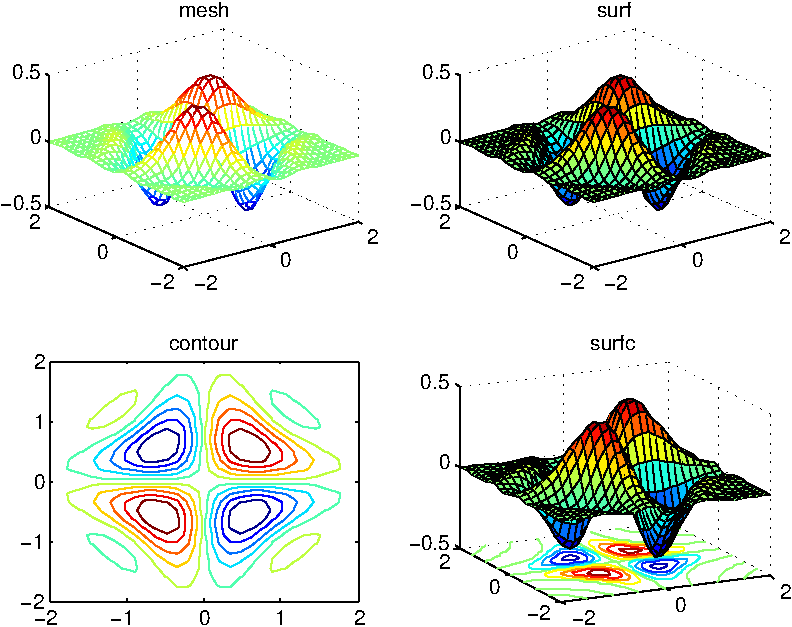
\includegraphics[width=0.8\textwidth]{figures/beispiel_function_plot_3d}\hfil
\end{frame}
% 
% Slide
% 
\begin{frame}[fragile]\frametitle{Funktionenplot - Implementation}
\begin{lstlisting}
% Erzeugen des Gitters
x = linspace(-2,2,30);
y = linspace(-2,2,30);
[X,Y] = meshgrid(x,y);
% Funktionswerte
Z = exp(-X.^2-Y.^2).*sin(pi*X.*Y);

% verschiedenen Darstellungen
subplot(2,2,1),
 mesh(X,Y,Z), title('mesh');
subplot(2,2,2),
 surf(X,Y,Z), title('surf');
subplot(2,2,3),
 contour(X,Y,Z,10), title('contour');
subplot(2,2,4),
 surfc(X,Y,Z);
 view(-26,20), title('surfc');
\end{lstlisting}
\end{frame}
% 
% Slide
% 
\begin{frame}[fragile]\frametitle{subplot}
\begin{lstlisting}
subplot(<n>,<m>,<k>)
\end{lstlisting}
zerlegt das Grafikfenster in $n \times m$ Teilfenster. 

Die Zahl $1
\leq k \leq nm$ gibt an, welches Teilfenster gerade aktiv
ist. \\

Durchnumeriert wird zeilenweise, also $(1,1), (1,2), \dots$.

\end{frame}

% 
% Slide
% 
\begin{frame}[fragile]\frametitle{meshgrid}
Zu Vektoren $x=(x_i)_{i=1}^k$, $y=(y_j)_{j=1}^n$ erzeugt 
\begin{lstlisting}
[X,Y]=meshgrid(x,y)
\end{lstlisting}
Matrizen $X,Y \in \mathbb{R}^{n \times k}$, wobei jede Zeile von $X$
eine Kopie des Vektors $x$ ist und $Y$ als Spalten den Vektor $y$
enthält. \\
Dann hat \alert{ \mcode{Z=X.*Y}} die Komponenten 
\[ Z(i,j)=x(j)*y(i). \]
\end{frame}
% 
% Slide
% 
\begin{frame}[fragile]\frametitle{Darstellungsmöglichkeiten}
% Das hier ist eigentlich doppelt..
\begin{itemize}
\item Contourplot (zeichnet die Niveaulinien): \alert{ \mcode{contour}}
\item Darstellung des Graphen mit Gitterlinien: \alert{ \mcode{mesh} ,
  \mcode{meshc}} 
\item Flächige Darstellung des Graphen: \alert{ \mcode{surf}, \mcode{surfc}}
\end{itemize} 

\alert{ \mcode{mesh(X,Y,Z)}} z.B. stellt für Matrizen $X,Y,Z \in
\mathbb{R}^{n \times k}$ die Punkte 
\[\alert{  (X(i,j), Y(i,j), Z(i,j))} \quad \mbox{dar.}\]
\end{frame}
% 
% Slide
% 
\begin{frame}[fragile]\frametitle{Weitere Möglichkeiten}
\begin{itemize}
\item Darstellung versteckter Linien (bei \mcode{mesh}): \alert{ \mcode{hidden off}}, Default:
\alert{ \mcode{hidden on}}
\item Verschmieren des Gitters: \alert{ \mcode{shading('interp')}}
\item Blickwinkel: \alert{ \mcode{view(az,el)}}
\item ähnlich wie \mcode{mesh}; nur mit 'Vorhang': \alert{
  \mcode{meshz(X,Y,Z)}}
\end{itemize}
\end{frame}
% 
% Slide
% 
\begin{frame}[fragile]\frametitle{Beispiel: Funktionenplot}
\hfil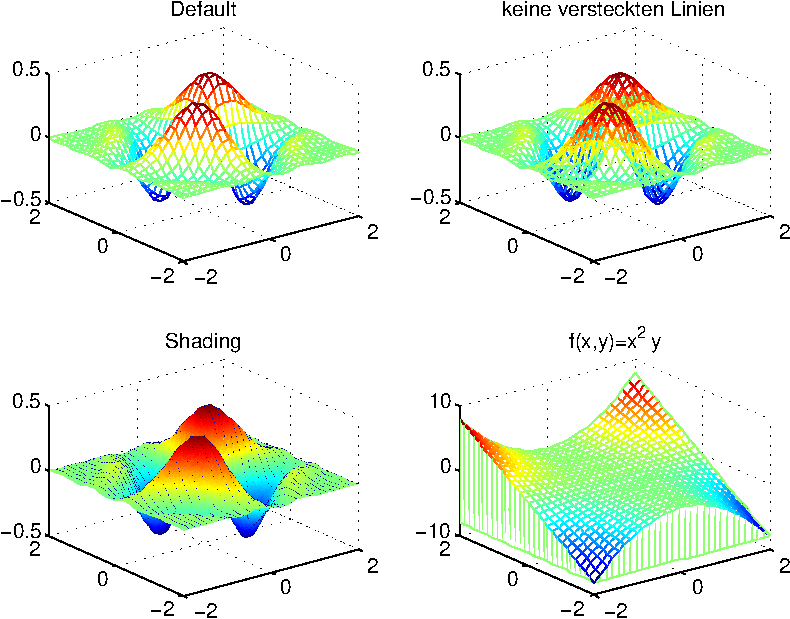
\includegraphics[width=0.8\textwidth]{figures/beispiel_function_plot_3d_2}\hfil
\end{frame}
% 
% Slide
% 
\begin{frame}[fragile]\frametitle{Programm}
\begin{lstlisting}
x = linspace(-2,2,30);
y = linspace(-2,2,30);
[X,Y] = meshgrid(x,y);
% Funktionswerte
Z = exp(-X.^2-Y.^2).*sin(pi*X.*Y);

% verschiedenen Darstellungen
subplot(2,2,1),
 mesh(X,Y,Z), title('Default');
subplot(2,2,2),
 mesh(X,Y,Z), hidden off,
 title('keine versteckten Linien');
subplot(2,2,3), surf(X,Y,Z);
 shading('interp'), title('Shading');
subplot(2,2,4), Z=X.^2.*Y;
 meshz(X,Y,Z), title('f(x,y)=x^2 y');
\end{lstlisting}
\end{frame}

% 
% Slide
% 
\begin{frame}[fragile]\frametitle{Contour Plots}
\hfil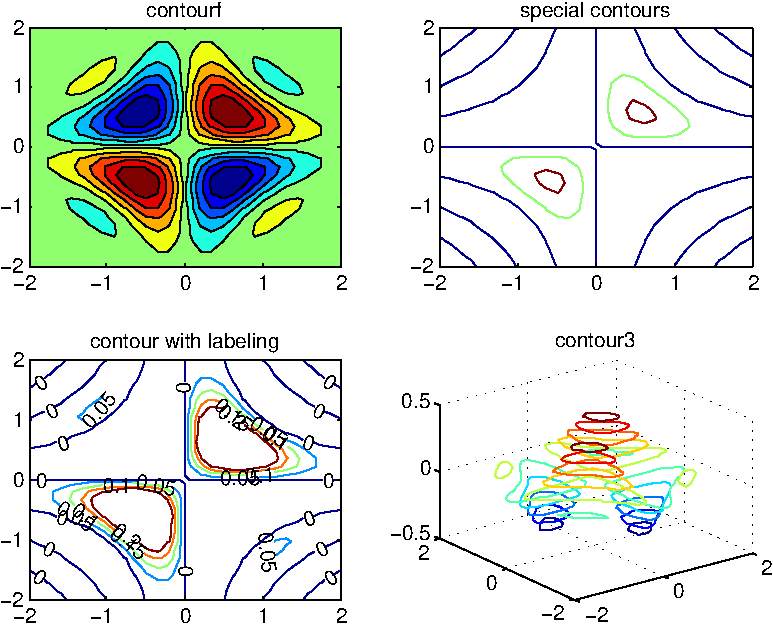
\includegraphics[width=0.8\textwidth]{figures/beispiel_function_plot_contour}\hfil
\end{frame}
% 
% Slide
% 
\begin{frame}[fragile]\frametitle{Contour Plots - Listing}
\lstinputlisting{contour_plot.m}
\end{frame}

% 
% Slide
% 
\begin{frame}[fragile]\frametitle{Erläuterungen zu Contour-Befehlen}
\begin{itemize}
\item \alert{\mcode{contour(X,Y,Z,n)}} zeichnet f\"ur $n\in \mathbb{N}$
  $n$-Konturlinien. Ist $n$ ein Vektor, werden Konturlinien zu den Werten in
  dem Vektor $n$ geplottet.
\item \alert{\mcode{contourf}} funktioniert wie \mcode{contour} nur das die Flächen
  zwischen den Konturlinien ausgefüllt werden.
\item \alert{\mcode{label(C,h)}} beschriftet die Konturlinien, deren Werte in $C$
  gespeichert sind und die zum Grafik-Handle $h$ gehören.
\item \alert{\mcode{contour3}} zeichnet jede Konturlinie auf einer anderen H\"ohe.
\end{itemize}
\end{frame}
%
% Slide
% 
\begin{frame}[fragile]\frametitle{Slice}
\begin{lstlisting}
slice(X,Y,Z,V,sx,sy,sz)
\end{lstlisting}
zeichnet  Schnitte zu den Funktionswerten $V(i)$ zu
$(X(i),Y(i),Z(i))$. Schnitte sind durch die Vektoren $sx$, $sy$ und $sz$
gegeben.\\
\textbf{Beispiel}: \alert{ \[ f(x,y,z):=\exp(-x^2-y^2)\sin(\pi x y z) \]}
\lstinputlisting{beispiel_slice.m}
\end{frame}

\begin{frame}[fragile]\frametitle{Beispiel: slice}
\hfil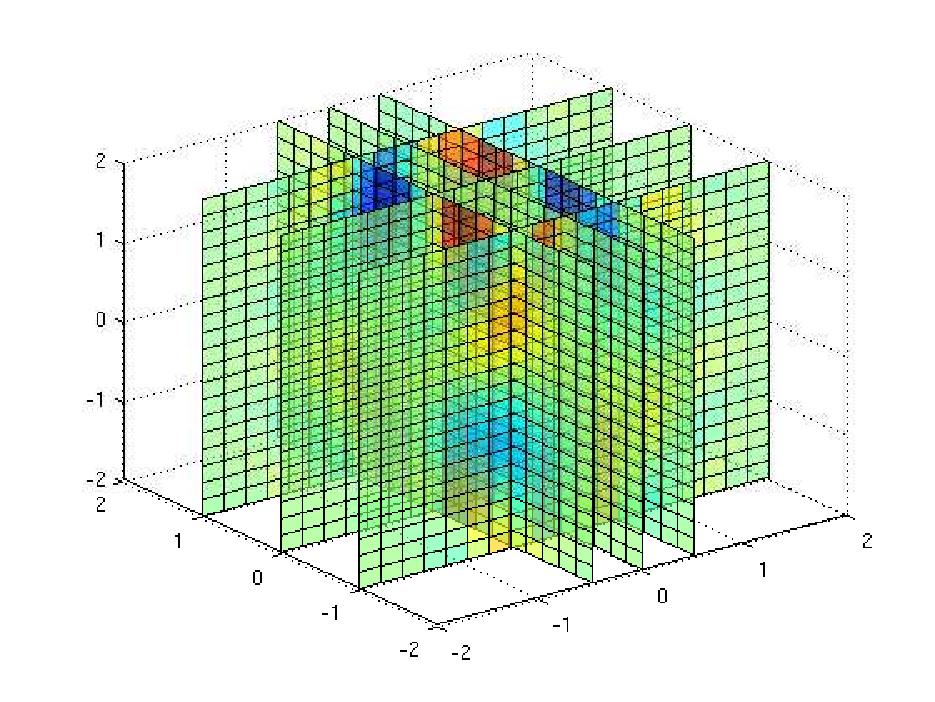
\includegraphics[width=0.8\textwidth]{figures/slice}\hfil
\end{frame}

\subsection{Animation}
% 
% Slide
% 
\begin{frame}[fragile]\frametitle{Animation-Beispiel}
\lstinputlisting{animation.m}
\end{frame}
%
% Slide
% 
\begin{frame}[fragile]\frametitle{Erstellen einer Animation}
\begin{itemize}
\item Mit \alert{\mcode{F(j)=getframe}} wird die aktuelle Grafik in das Array
  $F$ gespeichert.
\item Sequenz der Bilder $F$ darstellen: \alert{\mcode{movie(F,n,fps)}},
  wobei $n$ die Anzahl der Wiederholungen angibt und $fps$ der
  gezeigten Frames pro Sekunde entspricht (Default: $n=1$, $fps=12$). 

\item Speichern des Movies in AVI Format: \alert{\mcode{movie2avi(F,Dateiname)}}
\end{itemize}
\end{frame}

%
% Slide
%


\end{document}




